\documentclass[output=paper]{LSP/langsci}
\ChapterDOI{10.5281/zenodo.1228245} 
\author{Laura J. Downing \affiliation{Göteborgs universitet}}
\title{Differential object marking in {C}hichewa}
%\epigram{Change epigram in chapters/01.tex or remove it there}
\abstract{In most Bantu languages, an object prefix can occur on the
 verb. 
 In some Bantu languages, this object prefix has a purely
 anaphoric function, while in others it has an additional agreement
 function. Since \citeauthor{Bresnanetal1987Topic}, Chichewa (Bantu N.31
 Malawi) has been considered a textbook example of a language where  the object marker is “always an incorporated pronoun and never a non-referential marker of grammatical agreement" \citep[755]{Bresnanetal1987Topic}.
 That is, in order for an overt nominal phrase (DP) to co-occur in the same sentence
 with an object prefix, the DP must be a dislocated Topic. 
 Conversely, a dislocated object DP (a Topic) must be anaphorically
 bound to an object prefix. In this paper I present new Chichewa data
 showing that in modern colloquial Chichewa there is a
 human/non-human asymmetry in object marking. 
 Human object DPs commonly co-occur with an object prefix, whether the object is a  dislocated Topic or not, whereas non-human ones commonly do not
 co-occur with an object prefix, even when they are dislocated
 Topics. 
 I conclude that Chichewa shows differential object marking
 (or object indexation), as humanness is a more important condition
 on the occurrence of object prefixes than word order. The
 implications of the Chichewa (and other Bantu) data for recent
 proposals like \citet{Creissels2006Typology},
\citet{Dalrympleetal2011Objects} and \citet{Iemmolo2013Symmetric,Iemmolo2014Differential} about the diachronic development of DOM agreement systems from
 anaphoric Topic marking systems are discussed, and an alternative
 constraints-based account is proposed.}
\maketitle

\begin{document}


\section{Introduction}\label{02-do-sec:1}

Object markers, commonly found in \ili{Bantu} languages, are part of a
complex string of pre-stem verbal inflectional prefixes, which include
an obligatory subject prefix and tense-aspect-mood (TAM) prefixes.
Object markers, when they occur, are positioned immediately before the
verb stem, as illustrated in the \ili{Swahili} example below.\footnote{There
 are 500+ \ili{Bantu} languages spoken over a huge geographic area, so, not
 surprisingly, this generalization about the position of object
 markers does not hold for all \ili{Bantu} languages. Rather, it holds for
 the languages spoken in the eastern and southern parts of the \ili{Bantu}
 region. This paper concentrates on languages from this area. See
\citet{Martenetal2012Object} and \citet{Beaudoinetal2004Pronominal}
 for more discussion of the variation in the position of object markers.}
(The \isi{object marker} is bolded):

%TODO [cmld] War hier nicht a und b wie im Manuskript? So gewollt? -- Ich hab das mal geändert um die Kontrolle zu erleichtern. Ok so?
%DONE Irgendwie fand ich es inhaltlich idiotisch mit a und b, aber wir können es so erstmal lassen
\begin{exe}
\ex
\begin{xlist}
\ex
\label{02-do-ex:1}%Bantu
\textit{Structure of the \ili{Bantu} verb} \citep{Meeussen1967Bantu, Nurse2003Aspect}\\
Subject - TenseAspectMood - \textbf{(Object)} - [\textsubscript{Stem}Root (-Extensions)-Final Vowel

\ex
\label{02-do-ex:1b}%Swahili
\langinfo{Swahili}{Bantu}{\citealt[4]{Riedel2009Syntax}}\\
\gll A-li-\textbf{wa}-[\textsubscript{Stem}on-a.\\
\textsc{cl}1\textsc{sbj}-\textsc{pst}-\textsc{cl}2\textsc{obj}-see-\textsc{fv}\\
\glt ‘S/he (class 1) saw them (class 2).’
\end{xlist}
\end{exe}

\noindent The form of both subject and object markers is determined by the concord class of the noun they refer to. 
Each noun concord class is traditionally assigned a number. 
In the interlinear glosses in~\REF{02-do-ex:1b}, for example, \textsc{cl}1\textsc{sbj} labels a subject marker from class 1; \textsc{cl}2\textsc{obj} labels an \isi{object marker} from class 2.

As we can see in~\REF{02-do-ex:1b}, object markers can function like incorporated pronouns, performing the function of independent pronominal words in languages like English. 
Work like \citet{Givon1976Topic}, \citet{Bresnanetal1987Topic}, and \citet{Creissels2006Typology} indeed agrees that \ili{Bantu} object markers have most plausibly developed historically from the \isi{grammaticalization} of independent pronouns. 
\citet[44–45]{Creissels2006Typology} proposes that there are three stages in the further evolution of the function of object markers cross-linguistically:

\begin{exe}
\ex
\label{02-do-ex:2}%ObjectMarkers
\begin{description}[leftmargin=!, labelwidth=\widthof{Stage~III:}]
\item [Stage~II:] the \isi{object marker} has a \textit{purely anaphoric} function, as it cannot occur within the limits of the clause [TP/IP] containing an overt co-referential object DP.
\item [Stage~II:] the \isi{object marker} acquires an additional \textit{agreement} function, as it obligatorily occurs, even if the clause contains a co-referential object DP. It retains an anaphoric function as it can also represent, on its own, a co-referential DP that is not contained within the limits of the clause.
\item [Stage~III:] at this stage, the pronominal marker has a \textit{purely agreement} function, as it cannot represent on its own a co-referential DP not contained within the limits of the clause.
\end{description}
\end{exe}

Since \citet{Bresnanetal1987Topic}, \ili{Chichewa} (\ili{Bantu} N31 Malawi) has been considered a textbook example of a Stage~I language.
The \isi{object marker} is “always an incorporated pronoun [anaphor] and never a non-referential marker of grammatical agreement” \citep[755]{Bresnanetal1987Topic}. 
In order for an overt DP to co-occur in the same sentence with an \isi{object marker}, the DP must be a dislocated Topic in their analysis. 
Conversely, a dislocated object DP (a Topic) must be anaphorically bound to an \isi{object marker} \citep[749]{Bresnanetal1987Topic}.

In this paper I present new \ili{Chichewa} data showing that, in fact, modern colloquial \ili{Chichewa} is a Stage~II language, with a human/non-human asymmetry in object marking: human object DPs commonly co-occur with object marking, whereas non-human ones commonly do not. 
I conclude that \ili{Chichewa} shows differential object marking (or object indexation), as humanness is a more important condition on the occurrence of object markers than \isi{word order}.

\newpage 
The paper is organized as follows. 
First, in~\sectref{02-do-sec:2}, I review \citegen{Bresnanetal1987Topic} diagnostics for purely anaphoric status of object markers. 
In~\sectref{02-do-sec:3}, I show that \ili{Chichewa} fails all of these diagnostics. 
Finally, in~\sectref{Downing-Implications}, I discuss the implications of the \ili{Chichewa} (and other \ili{Bantu}) data for recent proposals like \citet{Creissels2006Typology}, \citet{Dalrympleetal2011Objects} and \citet{Iemmolo2013Symmetric,Iemmolo2014Differential} 
about the \isi{diachronic development} of DOM agreement systems and develop a constraints-based account.


\section{Diagnostics for the anaphoric vs. grammatical agreement function of object markers}\label{02-do-sec:2}

\subsection{Object marker is purely anaphoric}\label{02-do-sec:2-1}

\citet{Bresnanetal1987Topic} propose the following diagnostics that determine whether object markers are purely anaphors, referring to Topics and other DPs (nominal phrases) outside the clause in a particular language. 
(This corresponds to \citeauthor{Creissels2006Typology}'s \citeyear{Creissels2006Typology} Stage~I):

\begin{exe}
\ex
\label{02-do-ex:3}%Diagnostics
Diagnostics for anaphoric use of object markers:
\renewcommand{\theenumi}{\alph{enumi}}
\begin{enumerate}
\item Word order: the occurrence of the \isi{object marker} correlates with non-canoni\-cal \isi{word order}; more precisely, only dislocated DPs are resumed with object markers and dislocated DPs must be resumed with object markers.
\item Focused elements: cannot be referred to with an \isi{object marker}.
\item Prosody: an object DP resumed by an \isi{object marker} is considered anaphoric if the object is phrased separately from a preceding object-marked verb.
\end{enumerate}
\end{exe}

If the \isi{object marker} meets these tests, then the \isi{object marker} is anaphoric. 
Any overt object DP which co-occurs with an \isi{object marker} must be dislocated. 
Any dislocated object DP must be licensed with (anaphorically bound to) an \isi{object marker}. 
Object markers have been argued to have a primarily anaphoric function, using these sorts of criteria, in \ili{Bantu} languages like: Haya \citep{Byarushengoetal1977Haya}, \ili{Northern Sotho} \citep{Zerbian2006Expression}, Tswana \citep{Creissels2006Typology}, \ili{Zulu} \citep{Buell2005Issues,Chengetal2009Zulu,Schadeberg1995Object,vanderSpuy1993Dislocated,Zeller2012Object} and \ili{Swati} \citep{Martenetal2012Object}. 
Indeed, \citegen{Creissels2006Typology} claims that Stage~I object markers are very common in African languages generally.\footnote{See also \citegen{Riedel2009Syntax}, \citegen{Martenetal2012Object} and \citegen{vanderWal2015Bantu}
 recent cross-\ili{Bantu} surveys.} 
 
The diagnostics for purely anaphoric use of the \isi{object marker} are illustrated with data from \ili{Zulu} \citep{Chengetal2009Zulu}. 
Canonical \isi{word order} in \ili{Zulu} is: S V IO DO Oblique. 
As shown by the \ili{Zulu} data in~\REF{02-do-ex:4} and~\REF{02-do-ex:5}, both left and right dislocations of object DPs are easily elicited by asking content questions on a verb complement. 
Both the content question word or particle and the answer to the content question (which have inherent focus) must occur immediately after the verb. 
A non-focused verb complement must be displaced from its canonical postverbal position either to preverbal position or to a position following the element in   immediately after the verb position. 
Note that we find an obligatory \isi{object marker} referring to an object or \isi{direct object} which has been displaced from its canonical position.\footnote{The accent marks on vowels in the data indicate high tone; long vowels are indicated by doubling the vowel. 
In the morpheme glosses, numbers indicate noun concord class, following the standard \ili{Bantu} system adopted in work like \citet{Mchombo2004Syntax}. 
Dislocated elements are underlined, and object markers are bolded.}

\protectedex{
\begin{exe}
\ex
Zulu left dislocations\langinfo{}{Bantu}{author's elicitation notes}\\\label{02-do-ex:4}
\emph{Wh-questions}
\begin{xlist}
\exi{Q}
\gll (\ule{Ámá-bhayisékíl’} u\textbf{-wá}-níkée ó-baani)?\\
\textsc{cl6}-bicycle \textsc{2sgsbj}-\textsc{cl6obj}-give.\textsc{prf} \textsc{cl2}-who\\
\glt ‘Whom did you give bicycles to?’
\exi{A}	
\gll (\ule{Ámá-bhayisékiili}) (si\textbf{-wá}-níkée ábá-ntwaana).\\
\textsc{cl6}-bicycle \textsc{1plsbj}-\textsc{cl6obj}-give.\textsc{prf} \textsc{cl2}-child\\
\glt	‘We gave bicycles to the children.’
\end{xlist}
\end{exe}}

\protectedex{
\begin{exe}
\ex
Zulu right dislocations\langinfo{}{Bantu}{author's elicitation notes}\\\label{02-do-ex:5}
\emph{Wh-questions}
\begin{xlist}
\exi{Q}
\gll ((Ízí-vakáashi) (zí-\textbf{yí}-thengelée-ni) \ule{ímí-ndeni} \ule{yáazo)}?\\
\textsc{cl8}-visitors \textsc{cl8sbj}-\textsc{\textbf{cl4obj}}-buy.for.\textsc{prf}-what \textsc{cl4}-families \textsc{cl4}.their\\
\glt	‘What did the visitors buy for their families?’
\exi{A}
\gll ((Ízí-vakáshí 	zí-\textbf{yí}-thengelé ízí-nguubo) \ule{ímí-ndeni} \ule{yáazo).}\\
\textsc{cl8}-visitors \textsc{cl8sbj}-\textsc{\textbf{cl4obj}}-buy.for.\textsc{prf}	\textsc{cl10}-clothes \textsc{cl4}-families \textsc{cl4}.their\\
\glt	‘The visitors bought clothing for their families.’
\end{xlist}
\end{exe}}

Evidence that the objects resumed with an \isi{object marker} (underlined) in~\REF{02-do-ex:5} are dislocated is that, first, they are set off prosodically from the rest of the sentence. 
As \citet{Chengetal2009Zulu} show, the main evidence for the prosodic phrasing (indicated by parentheses) is lengthening of the phrase penult vowel. 
(Vowel length is not contrastive in \ili{Zulu}.) 
Furthermore, IO DO \isi{word order} is strictly respected in broad focus sentences. 
The DO IO order in~\REF{02-do-ex:5} is only felicitous if the DO is in focus and IO is out of focus. 
As \citet{Chengetal2009Zulu} and \citet{Kucerovaetal2012Against} argue, non-focused material cannot occur within the \textit{v}P in Durban \ili{Zulu}.
While dislocated objects must be resumed with an \isi{object marker}, objects in focus (and therefore in IAV position) cannot be resumed with an \isi{object marker}. 
This is shown by the infelicitous sentence in~\REF{02-do-ex:6c}, where the \isi{object marker} \textit{zi-} refers to ‘visitors’, the word in focus, rather than to ‘chicken’, old information repeated from the question (and dislocated out of the vP):

\protectedex{
\begin{exe}
\ex
\label{02-do-ex:6}
\langinfo{Zulu}{Bantu}{author's elicitation notes}

\begin{xlist}
\exi{a. Q}\label{02-do-ex:6a}

\gll ((Ú-siipho) (ú-\textbf{yí}-phékéla BAANI) \ule{ín-kuukhu)}?\\
\textsc{cl1}-Sipho	 \textsc{cl1sbj}-\textsc{\textbf{cl9obj}}-cook.for \textsc{cl1}.who \textsc{cl9}-chicken\\
\glt	‘Who is Sipho cooking the chicken for?’
	
\exi{b. A}\label{02-do-ex:6b}
  \gll 	((Ú-síph’ ú-\textbf{yí}-phékél’ ÍZÍ-VAKÁASH’) \ule{ín-kuukhu)}.\\
\textsc{cl1}-Sipho \textsc{cl1sbj}-\textsc{\textbf{cl9obj}}-cook.for \textsc{cl8}-visitor \textsc{cl9}-chicken\\
\glt	‘Sipho is cooking the chicken for the visitors.’

\ex \label{02-do-ex:6c}
\gll	\#Ú-síph’ ú-\textbf{zí}-phékél’ ÍZÍ-VAKÁASH’ ín-kuukhu.\\
\textsc{cl1}-Sipho	 \textsc{cl1sbj}-\textsc{\textbf{cl8obj}}-cook.for \textsc{cl8}-visitor \textsc{cl9}-chicken\\
\end{xlist}
\end{exe}
}

(Object marking would only be acceptable with the \isi{word order} in~\REF{02-do-ex:6c} as the answer to a question like, “What did Sipho do with the chicken for the visitors?” where ‘visitors’ is topical, given information.) 
The data set in~\REF{02-do-ex:6} demonstrates especially clearly that in \ili{Zulu} we find the correlation between \isi{object marker} and topical (or dislocated, out of focus) status of the co-referential object that \citet{Bresnanetal1987Topic} and \citet{Creissels2006Typology} have proposed characterize the \isi{object marker} in languages where it has a purely anaphoric function. 
(This corresponds to \citealt{Creissels2006Typology}'s Stage~I.)\footnote{Though \citet{Zeller2012Object} provides some problematic examples, showing humanness plays a role in object marking in \ili{Zulu} for some speakers in some grammatical contexts, the consensus in the \ili{Zulu} literature is that object marking correlates with dislocation of the object DP. 
See \citet{vanderSpuy1993Dislocated,Chengetal2009Zulu,Schadeberg1995Object}, and \citet{Buell2005Issues} for discussion.}


\subsection{Object marker is also a grammatical agreement marker}
\label{02-do-sec:2-2}

As far as I know, in all \ili{Bantu} languages, the \isi{object marker} can have an anaphoric (pronominal) function, resuming objects that occur earlier in the discourse as well as (at least some) topical, dislocated objects. 
The \isi{object marker} also has a grammatical agreement-like function in some \ili{Bantu} languages: it can co-occur with a co-referential object within the same TP/IP (i.e., roughly, a clause).\footnote{See \citegen{Morimoto2002Prominence}, \citegen{Riedel2009Syntax}, \citegen{Martenetal2012Object} and \citegen{vanderWal2015Bantu} recent surveys of the variation in the function and distribution of pre-verb stem object markers, illustrating a range of possibilities from \citet{Creissels2006Typology} Stage~I to Stage~II. 
(As \citealt{Creissels2006Typology} notes, Stage~III is not common in the languages of the world.)} 
Languages where this has been demonstrated include Bemba \citep{Martenetal2012Object}, \ili{Swahili}, Sambaa, Chaga \citep[59]{Riedel2009Syntax}, Chimwiini \citep{Kisseberthetal1977Chimwini} and \ili{Manyika Shona} \citep{Baxetal2012Information}. 
For example, in \ili{Swahili}, as we saw in~\REF{02-do-ex:1b} object markers can serve an anaphoric function, resuming objects mentioned earlier in the discourse. 
They also serve a grammatical agreement function: object marking is obligatory with overt human objects – \REF{02-do-ex:7a} – and common with \isi{definite} non-human objects – \REF{02-do-ex:7c}:\footnote{Object marking might not be as obligatory in colloquial \ili{Swahili} as traditionally described, see \citet{Seidletal1997Discourse} for discussion.} 
 
\protectedex{
\ea \label{02-do-ex:7}
\langinfo{Swahili}{Bantu}{\citealt[42, 46]{Riedel2009Syntax}}

\ea \label{02-do-ex:7a}
\gll	Ni-li-\textbf{mw}-ona mwanawe.\\
\textsc{1sgsbj}-\textsc{pst}-\textsc{cl1obj}-see \textsc{cl1}.child.\textsc{poss.3sg}\\
\glt	‘I saw his child.’

\ex \label{02-do-ex:7b}
\textit{*Ni-li-ona mwanawe}\\

\ex \label{02-do-ex:7c}
\gll	Ni-li-\textbf{zi}-ona picha hizo.\\
 \textsc{1sgsbj}-\textsc{pst}-\textsc{cl10obj}-see \textsc{cl10}.picture \textsc{cl10}.those\\
\glt	‘I saw those pictures.’	
\z
\z
}

\citet{Riedel2009Syntax} affirms that the \isi{object marker} in these examples occurs even though the overt object is in its base position, and no prosodic break separates the object-marked verb from the overt object.
\ili{Bantu} languages with grammatical agreement-like object marking show a great deal of variation as to whether the markers are obligatory or optional. 
The unifying generalization is that agreement-like object markers co-occur with human or \isi{animate} objects or with \isi{definite} objects. 
(See, \eg \citealt{Duranti1979Object,Bentley1994Syntactic,Morimoto2002Prominence, Riedel2009Syntax,Martenetal2012Object,vanderWal2015Bantu}). 
That is, agreement-like marking of objects in \ili{Bantu} languages is conditioned by the \isi{topicality} hierarchies in~\REF{02-do-ex:8}:\footnote{See \citetv{Witzlacketal2017Differential} for a detailed overview of the role of different versions of the hierarchies in~\REF{02-do-ex:8} in accounting for DOM. 
While the term \emph{\isi{topicality} hierarchy} is well-established in the literature, a number of other terms are also in current use, as \citetv{Witzlacketal2017Differential} make clear.}

\ea \label{02-do-ex:8}
Topicality hierarchies (\citealt[224]{Hymanetal1982Bantu})
\renewcommand{\theenumi}{\alph{enumi}}
\begin{enumerate}
\item Benefactive > Recipient > Patient > Instrument
\item 1\textsuperscript{st} > 2\textsuperscript{nd} > 3\textsuperscript{rd} human > 3\textsuperscript{rd} animal > 3\textsuperscript{rd} \isi{inanimate}
\item \isi{definite} > \isi{indefinite}
\end{enumerate}
\z

\noindent These hierarchies have also been shown to play a central role in defining other object properties in \ili{Bantu} languages \citep{Duranti1979Object, Hymanetal1974Hierarchies, Hymanetal1982Bantu}, and in conditioning differential object marking in a number of typologically diverse languages. 
(See \eg \citealt{Comrie1981Language, Comrie1989Language,Aissen2003Differential,Iemmolo2013Symmetric,Iemmolo2014Differential}). 
\citet[48--49]{Creissels2006Typology} qualifies \ili{Bantu} languages like \ili{Swahili} as in transition from Stage~I to Stage~II because agreement object markers are not entirely obligatory. 
This is because only some types of objects – human and \isi{definite} – show agreement-like object marking in \ili{Swahili}. 
He notes that pure Stage~II object marking systems are not common in African languages, but provides no explanation for why this might be so. 
I take up the discussion of how languages might change from anaphoric object marking to a system of differential grammatical agreement object marking in~\sectref{Downing-Implications}. 
First, I review the distribution of object marking in modern colloquial \ili{Chichewa}.

\section{The function of object markers in Chichewa: anaphoric or grammatical agreement?}\label{02-do-sec:3}

As noted above, since \citet{Bresnanetal1987Topic}, \ili{Chichewa} is considered to be a prototypical Stage~I language: the \isi{object marker} is always an anaphor and signals that the cooccurring object does not occur within the same VP as the \isi{object marker}. 
Furthermore, dislocated objects must be resumed by an \isi{object marker}. 
Recall that these claims about the pronominal status of the \isi{object marker} are based on the diagnostics in~\REF{02-do-ex:3}. 
In this section, I present new \ili{Chichewa} data, recently elicited in Malawi.\footnote{The data was collected using an elicitation questionnaire for an investigation that had as its original aim to describe the prosody of dislocated nominals.
However, once I noticed that the use of object markers did not match \citegen{Bresnanetal1987Topic} description, I re-elicited data from \citet{Bresnanetal1987Topic} to test their diagnostics for the distribution of object markers on this set of speakers. 
The elicitation interviews were conducted in Malawi in 2011 and 2013, primarily with four native speakers of \ili{Chichewa} aged between 22 and 40 years old. 
The resulting corpus investigating the distribution of object markers consists of some 50–75 sentences per speaker. 
Pascal Kishindo, Professor of \ili{Chichewa} syntax at Chancellor College and a native speaker of \ili{Chichewa}, kindly checked the corpus and has confirmed that all the examples cited in this section are grammatical.} 
As we will see, object marking in modern colloquial \ili{Chichewa} fails all three of \citegen{Bresnanetal1987Topic} diagnostics for anaphoric status. 
Instead, it shows differential object marking properties. 
I take up \citegen{Bresnanetal1987Topic} diagnostics one by one below.

\subsection{Changes in word order and object marking}\label{02-do-sec:3-1}

In \ili{Chichewa}, as in most \ili{Bantu} languages, the basic \isi{word order} is: (Subject) Verb (Object1) (Object2) (Oblique). 
(See, \eg \citealt{Heine1976Typology,Bearth2003Syntax, Downingetal2016Information}). 
\ili{Chichewa} allows multiple objects, with a non-theme (\eg benefactive) object generally preceding the theme object.
Adverbials and other oblique arguments are found at the periphery of the main clause. 
According to \citet{Mchombo2004Syntax}, nothing can separate an object nominal from the preceding verb, unless the verb is object-marked.

In my corpus one frequently finds examples where a co-referential \isi{object marker} on the verb resumes a dislocated object DP. 
(Parentheses continue to indicate prosodic phrasing.)\footnote{See \citet{Chengetal2016Phasal} for justification of the prosodic phrasing indicated in these examples.}
This data is consistent with \citegen{Bresnanetal1987Topic} diagnostics for the purely anaphoric status of object marking given in~\REF{02-do-ex:3}:

%\protectedex{
\ea Left dislocations\\
\langinfo{Chichewa}{Bantu}{author's elicitation notes} 
\ea\label{02-do-ex:9}

\gll ((\ule{Chi-máangá}) (á-\textbf{chí}-lima nyengo í-kú-bwélaa-yi) ((ndipó \ule{fóodya}) (a-dzá-\textbf{mú}-lima nyengo ínáayo).\\
		\textsc{cl7}-maize \textsc{cl1sbj.pst}-\textsc{cl7obj}-cultivate \textsc{cl9}.season \textsc{cl9}-\textsc{prog}-come-\textsc{cl9.rel} and \textsc{cl3}.tobacco \textsc{cl1sbj}-\textsc{fut}-\textsc{cl3obj}-cultivate \textsc{cl9}.season \textsc{cl9}.next\\
\glt ‘Maize she cultivated this season, and tobacco she will cultivate next season.’
	
\ex\label{02-do-ex:10}
\gll (\ule{Mwaná} 	\ule{wódwálaa-yo}) (á-kú-\textbf{mu}-téngéla ku chipataalá) (ndi ndaání).\\
	\textsc{cl1}.girl \textsc{cl1}.sick-\textsc{cl1dem} \textsc{cl1sbj}-\textbf{\textsc{prog}}-\textsc{cl1obj}-take.to \textsc{loc} \textsc{cl7}.hospital \textsc{cop} who\\
\glt ‘That sick child, (the one) taking her to the hospital is who?’
\z
\z
%}
\ea\label{02-do-ex:11}
Right dislocations\\
\langinfo{Chichewa}{Bantu}{author's elicitation notes}
\ea \label{02-do-ex:11a}
\gll (((Pa tébuuló) (wa-\textbf{zí}-ika) mtsíkaana) \ule{mbaale}).\\
		\textsc{loc} \textsc{cl5}.table \textsc{cl1sbj.pst}-\textsc{cl10obj}-put \textsc{cl1}.girl		 \textsc{cl10}.plate\\
\glt ‘On the table, [she] put them, the girl, plates.’

\ex
\label{02-do-ex:11b}%ChichewaRight
\langinfo{Chichewa}{Bantu}{author's elicitation notes}

\gll ((((Udzuúdzú) (u-na-\textbf{wá}-lúmá kwámbíili) 	pa nyaánjá) 	dzuuló) a-soodzi).\\
\textsc{cl14}.mosquito \textsc{cl14sbj}-\textsc{pst}-\textsc{cl2obj}-bite much \textsc{loc} \textsc{cl9}.lake yesterday \textsc{cl2}-fisherman\\
\glt ‘The mosquitoes bit them a lot on the lake yesterday, fishermen.’
\z
\z

\noindent We find many examples, though, where the occurrence of the \isi{object marker} does not correlate with dislocation of the co-referential DP. 
Human objects are often resumed by an \isi{object marker}, even when they are in their base position, immediately following the verb. 
In \REF{02-do-ex:12}, the same sentence is given with four different word orders. 
Note that no prosodic break separates the overt object from the verb in these examples, and there is no other evidence that the overt object is dislocated in any of the sentences:\footnote{I am not the first to observe that object markers can co-occur with in situ (human) objects in \ili{Chichewa}. 
Indeed, \citet{Bresnanetal1987Topic} mention this possibility in a footnote. 
\citet{Bentley1994Syntactic} and \citet{Henderson2006Syntax} also provide a few examples. 
As far I know, this paper is, though, the first attempt to systematically document the role of humanness in conditioning object marking in \ili{Chichewa}.} 

\protectedex{
\begin{exe}
\ex
\label{02-do-ex:12}%Chichewareelicited
\langinfo{Chichewa}{Bantu}{data re-elicited from \citealt{Bresnanetal1987Topic}}
\begin{xlist}

\ex
\label{02-do-ex:12a}%Chichewareelicited
\gll (Njúuchí) 	(zi-na-lúmá a-leenje).\\
	\textsc{cl10}.bee \textsc{cl10sbj}-\textsc{pst}-bite \textsc{cl2}-hunter\\

\ex \label{02-do-ex:12a2}
\gll (Njúuchí) 	(zi-na-\textbf{wá}-lúma 					a-leenje).\\
	\textsc{cl10}.bee \textsc{cl10sbj}-\textsc{pst}-\textsc{cl2obj}-bite \textsc{cl2}-hunter\\

\ex
\label{02-do-ex:12b}%Chichewareelicited
\gll ((Zi-na-lúmá a-leenje) njúuchi).\\
	\textsc{cl10sbj}-\textsc{pst}-bite \textsc{cl2}-hunter \textsc{cl10}.bee\\

\ex \label{02-do-ex:12b2}
\gll ((Zi-na-\textbf{wá}-lúma a-leenje) njúuchi).\\
	\textsc{cl10sbj}-\textsc{pst}-\textsc{cl2obj}-bite \textsc{cl2}-hunter \textsc{cl10}.bee\\
\glt ‘The bees bit the hunters.’\\
\end{xlist}
\end{exe} 
}
\newpage 

The point they illustrate is that it is acceptable for the \isi{object marker} \textit{wa-} to co-occur with the object it refers to, ‘hunters’. 
Both the sentences containing \textit{wa-} – \REF{02-do-ex:12a2} and \REF{02-do-ex:12b2} – and the ones omitting it – \REF{02-do-ex:12a} and \REF{02-do-ex:12b} – are judged grammatical by all the speakers I have asked, even though, according to \citet{Bresnanetal1987Topic}, the versions with the \isi{object marker} should not be acceptable.
More examples of the use of object markers with in situ objects are given below. 
(Note that in \ili{Chichewa}, unlike in \ili{Zulu}, objects in focus are not required to occur in immediately after the verb position):

\ea\label{02-do-ex:13}%Chichewa
\langinfo{Chichewa}{Bantu}{author's elicitation notes}\\ 

\gll (M-zákee-yó) (a-na-\textbf{mú}-pátsá Málíya chóóváala).\\
	\textsc{cl1}-friend-\textsc{cl1dem} \textsc{cl1sbj}-\textsc{pst}-\textsc{cl1obj}-give \textsc{cl1}.Mary \textsc{cl7}.dress\\
\glt ‘Her friend gave Mary a dress.’
\z

\ea\label{02-do-ex:14}%Chichewa
\langinfo{Chichewa}{Bantu}{\citealt[84, 91]{Downingetal2011Prosodic}}
\ea
\label{02-do-ex:14a}%Chichewa
\gll (Ndi zóóváala) (zi-méné a-lendó á-ná-\textbf{mu}-gulílá m-phunzitsii-zo).\\ 
	\textsc{cop}	\textsc{cl8}.clothes \textsc{cl8}-\textsc{rel} \textsc{cl2}-visitor \textsc{cl2sbj}-\textsc{pst}-\textsc{cl1obj}-buy.for \textsc{cl1}-teacher-\textsc{cl8}.\textsc{rel}\\
\glt ‘It is clothes that the visitors bought for the teacher.’

\ex
\label{02-do-ex:14b}%Chichewa
\gll ((Ti-na-kúmána 	nd’ áá-méné á-ná-\textbf{mu}-óná Báanda) dzuulo).\\
	we-\textsc{pst1}-meet with \textsc{cl2}-\textsc{rel} \textsc{cl2sbj}-\textsc{pst}-\textsc{cl1obj}-see	\textsc{cl1}.Banda yesterday\\
\glt ‘We met the ones who saw Banda yesterday.’
\z
\z

Human objects are commonly resumed with an \isi{object marker} whether they precede or follow a content question word like \textit{chiyáani} ‘what’; \isi{word order} has no effect on the occurrence of object marking:

\begin{exe}
\ex
\label{02-do-ex:15}%Chichewa
\langinfo{Chichewa}{Bantu}{author's elicitation notes}
\begin{xlist}

\ex
\label{02-do-ex:15a}%Chichewa
\gll ((Mu-ku-\textbf{wá}-phíkila chiyáani) aáná)?\\
	you-\textsc{prog}-\textsc{cl2obj}-cook.for	what \textsc{cl2}.children\\

\ex
\label{02-do-ex:15b}%Chichewa
\gll ((Mu-ku-\textbf{wá}-phíkila aáná) chiyáani)?\\
	you-\textsc{prog}-\textsc{cl2obj}-cook.for	\textsc{cl2}.children what\\
\glt ‘What are you cooking for the children?’
\end{xlist}
\end{exe}

Another problem for the anaphoric status of object markers posed by this data is that non-human objects are not systematically resumed with an \isi{object marker}. 
This is true even in contexts where they meet diagnostics for dislocation, such as preverbal position:

\newpage 
\begin{exe}
\ex
\label{02-do-ex:16-18}%Chichewa
\emph{Preverbal objects}\\
\langinfo{Chichewa}{Bantu}{author's elicitation notes}
\begin{xlist}
\ex %(16)
\label{02-do-ex:16}
\gll ((U-nga-kumbukila 	kútí 	búkuu-li)				a-ná-gulá-di 				ku 	Blántaayá)?\\
	 you-can-remember	 	that	\textsc{cl5}.book-\textsc{cl5}.this		\textsc{cl1sbj}-\textsc{pst}-buy-\textsc{emph}	\textsc{loc} 	Blantyre\\
\glt ‘Can you remember whether she bought this book in Blantyre?’
	

\ex %(17)
\label{02-do-ex:17}
\gll (Chí-mánga 	á-líma 					ch-aka 		ch-iinó) 		(ndipó 	fódya a-dzá-líma 				ch-aka 		chá 		máawa).\\
\textsc{cl7}-maize		\textsc{cl1sbj}.\textsc{pst}-cultivate	\textsc{cl7}-season	\textsc{cl7}.this		 and		\textsc{cl5}.tobacco	\textsc{cl1sbj}-\textsc{fut}-cultivate 	\textsc{cl7}-season	\textsc{cl7}.of	next\\
\glt ‘Maize, she will cultivate this season, and tobacco she will cultivate next season.’ (cf.~\REF{02-do-ex:9})

\ex%(18)
\label{02-do-ex:18}
\gll (Kodí		makáala) 		(u-náa-gula 	kuuti)?\\
\textsc{q}			\textsc{cl6}.charcoal	you-\textsc{pst}-buy	where\\
\glt 	‘Where did you buy charcoal?’
\end{xlist}
\end{exe}

Non-human objects are also not necessarily resumed with an object
marker when they follow a postverbal temporal adjunct. This is another
position where they are clearly dislocated, since objects otherwise
cannot be separated from the verb by an adjunct in \ili{Chichewa}
\citep{Mchombo2004Syntax}:\footnote{The attentive reader will have noticed that there are a number of different past tenses, all labeled \textsc{pst}. I have
 not labeled them more specifically, as choice of tense does not
 condition object marking.}
 
\begin{exe}
\ex
\label{02-do-ex:19-20:Chichewa}
\emph{Postverbal, post adjunct object}\\
\langinfo{Chichewa}{Bantu}{author's elicitation notes}
\begin{xlist}

\ex 	\emph{Context: ‘When will s/he write a 	 to the school?} %(19)

\gll ((A-dzá-lémba 		máawá) 		káláta 		yópítá 			ku 	sukúulu).\\
	 \textsc{cl1sbj}-\textsc{fut}-write		tomorrow	\textsc{cl9}.letter		\textsc{cl9}.of.\textsc{inf}.go	\textsc{loc}	\textsc{cl5}.school\\
\glt ‘S/he will write a letter to the school tomorrow.’

\ex 	\emph{Context: Can you also play the drums?} %(20)

\gll (Íinde) 	(ndí-ma-yímba 	BWINO 	\ule{ng’ooma}).\\
	 yes		I-\textsc{hab}-play			well		\textsc{cl10}.drum\\
\glt ‘Yes, indeed, I play the drums well.’
\end{xlist}
\end{exe}

In some cases, a consultant would even pronounce the verb with and without the \isi{object marker} in successive repetitions of the same sentence:

{
\begin{exe}
\ex
\label{02-do-ex:21}%Chichewa
\langinfo{Chichewa}{Bantu}{author's elicitation notes}
\begin{xlist}

\ex \emph{Context: Where did you buy the charcoal?}

%(20a)
\gll ((Ta-gula 			KU MSIIKÁ) 			\ule{makáala}).\\
	 we.\textsc{pst}-buy	\textsc{loc} \textsc{cl3}.market		\textsc{cl6}.charcoal\\

\ex 
\gll ((Ta-wá-gula 			KU MSIIKÁ) 		\ule{makáala}).\\
	 we.\textsc{pst}-\textsc{cl6obj}-buy	\textsc{loc} \textsc{cl3}.market		\textsc{cl6}.charcoal\\
\glt ‘We bought the charcoal at the market.’
\end{xlist}
\end{exe}
}
Following a content question word (or other word) in immediately after the verb position (indicated with capital letters), an \isi{object marker} is again not obligatory for a non-human object:

\begin{exe}
\ex
\label{02-do-ex:22}%Chichewa
\langinfo{Chichewa}{Bantu}{author's elicitation notes}
\begin{xlist}

\ex 
\gll (((Kodí 	azi-bambo 		a-na-nyámúla 		BWÁANJI)	 \ule{makáala}) 		ku msiika)?\\
	 \textsc{q}		\textsc{cl2}-man			\textsc{cl2.sbj.pst}-carry	how			\textsc{cl6}.charcoal	\textsc{loc} \textsc{cl3}.market\\
\glt ‘How did the men carry the charcoal to market?’

\ex 
\gll (((Kodí 	m-tsíkana 	a-naká-chápá 		KUUTI) 	zóoválá 		zá 	 		á-máy’ 		aáké)?\\
	 \textsc{q}		\textsc{cl1}-girl		\textsc{cl1sbj}-\textsc{pst}-wash	where		\textsc{cl8}.clothes 	\textsc{cl8}.of	\textsc{cl2}-mother	\textsc{cl2}.her\\
\glt ‘Where did the girl wash her mother’s clothes on Sunday?’
\end{xlist}
\end{exe}

According to my language consultants, there is no difference in interpretation, whether the \isi{object marker} is present or not.
This overabundance of human object marking compared to non-human is also found in relative clauses. 
As studies of \ili{Chichewa} relative clauses like \citet{Downingetal2011Prosodic}, \citet{Henderson2006Syntax},
 and \citet{Mchombo2004Syntax} show, human \isi{indirect object} heads are obligatorily resumed with object marking on the relative verb \REF{02-do-ex:23a}; human \isi{direct object} heads are commonly resumed \REF{02-do-ex:23b}; while non-human \isi{direct object} heads are not resumed \REF{02-do-ex:23c}. 
(The facts regarding non-human \isi{indirect object} heads need further study.)

{
\begin{exe}
\ex
\label{02-do-ex:23}%Chichewa
\langinfo{Chichewa}{Bantu}{\citealt{Downing2010Prosodic}, \citealt[76, 78]{Downingetal2011Prosodic}. The RC is underlined.}

\begin{xlist}

\emph{Human head of RC – object marking}

\ex \label{02-do-ex:23a}%Chichewa%23a
\gll ((\ule{A-lendó} 		\ule{a-méné} 	\ule{á-ná-wa-bweretsérá} \ule{m-pháatso}) 	a-koondwa).\\
	 \textsc{cl2}-visitor		\textsc{cl2}-\textsc{rel} 	\textsc{cl2sbj}-\textsc{pst}-\textsc{cl2obj}-bring.for		\textsc{cl10}-gift		\textsc{cl2sbj}-be.happy\\
\glt ‘The visitors who they brought the gifts for are happy.’

\ex \label{02-do-ex:23b}%Chichewa%23b
\gll ((\ule{A-lendó} 	\ule{a-méné} 	\ule{Bándá} 		\ule{á-ná-wá-óná} 				\ule{ku} 	\ule{sukúulu})		a-pìítá).\\
	 \textsc{cl2}-visitor	\textsc{cl2}-\textsc{rel}	\textsc{cl1}.Banda	\textsc{cl1sbj}-\textsc{pst}-\textsc{cl2obj}-see	\textsc{loc} 	\textsc{cl5}.school	\textsc{cl2sbj}-go\\
\glt ‘The visitors who Banda saw at the school have gone.’
\\
\emph{Non-human head of RC – no object marking}

\ex \label{02-do-ex:23c}%Chichewa%23c
\gll ((M-waná 	wá súkúlú 		a-ná-lémba 				\ule{káláta} \ule{i-méné} \ule{m-phunzitsi}	\ule{á-ná-weléenga})	kwá 	a-nyúuzi).\\
	 \textsc{cl1}-child	\textsc{cl1}.of school	\textsc{cl1sbj}-\textsc{pst}-write		\textsc{cl9}.letter \textsc{cl9}-\textsc{rel}	\textsc{cl1}-teacher \textsc{cl1sbj}-\textsc{pst}-read	for		\textsc{cl2}-newspaper\\
\glt ‘A student wrote the letter which the teacher read for the newspaper.’
\end{xlist}
\end{exe}
}

\subsection{Object markers and focus}\label{02-do-sec:3-2}

As \citet{Bresnanetal1987Topic} argue, if the \isi{object marker} in \ili{Chichewa} were a Stage~I, purely anaphoric agreement marker, it should never be co-referential with an element in focus. However, we find object marking for human words in focus: \eg content question words and the answers to content questions, as shown by the data below:

\begin{exe}
\ex
\label{02-do-ex:24}
\langinfo{Chichewa}{Bantu}{author's elicitation notes}
\begin{xlist}

\ex \label{02-do-ex:24a}
\gll (Kodí) 	((u-na-\textbf{mú}-óná 	NDAÁNI) 	ku 	tchálítchi 		m’máawá)?\\
	\textsc{q}	 \textsc{2sgsbj}-\textsc{pst}-\textsc{cl1obj}-see	\textsc{cl1}.who		\textsc{loc}	\textsc{cl5}.church		\textsc{loc}.morning\\
\glt ‘Who did you see at church in the morning?’

\ex \label{02-do-ex:24b}
\gll \emph{Q} (Kodí 	ámáyi		a-ná-\textbf{m}-pátsá		NDANÍ ma-lalaanje)?\\
{ } \textsc{q}	\textsc{cl2}.mother	\textsc{cl2sbj.pst}-\textsc{cl1obj}-give	\textsc{cl1}.who		\textsc{cl6}-orange?\\
\glt ‘Who did mother give the oranges to?’%TODO check why the translation is separated by a line break

\ex \label{02-do-ex:24c}
\gll \emph{A}	((Amáayi) 		(a-ná-\textbf{m}-pátsá					NZÁAWO) 			ma-lalaanje).\\
 { } \textsc{cl2}.mother	\textsc{cl2sbj.pst}-\textsc{cl1obj}-give	\textsc{cl1.poss}.friend	\textsc{cl6}-orange\\
\glt ‘Mother gave her friend the oranges.’%TODO check why the translation is separated by a line break

\end{xlist}
\end{exe}

Note in the following example that the dislocated non-human object \textit{kalata-yo} is not resumed with an \isi{object marker}, while the in situ, focused human object \textit{Prisca} is:

\begin{exe}
\ex
\label{02-do-ex:26}%Chichewa
\langinfo{Chichewa}{Bantu}{author's elicitation notes}

\emph{Context: ‘Who did the teacher write the letter to?’} 

\gll (Kálátaa-yó) 		(a-ná-\textbf{mú}-lémbera 				PRÍSCA).\\
	\textsc{cl9}.letter-\textsc{dem} \textsc{cl1sbj}-\textsc{pst}-\textsc{cl1obj}-write.to	\textsc{cl1}.Prisca\\
\glt ‘That letter, the teacher wrote to Prisca.’
\end{exe}

The by now familiar human vs. non-human asymmetry in object marking also holds in this focus context. It is considered ungrammatical to use an \isi{object marker} with a non-human content question word:

\begin{exe}
\ex
\label{02-do-ex:27}%Chichewa
\langinfo{Chichewa}{Bantu}{author's elicitation notes}
\begin{xlist}

\ex \label{02-do-ex:27a}%Chichewa
\gll (Kodí 	mu-ku-fúná 		chiyáani)?\\
	\textsc{q}	\textsc{2sgsbj}-\textsc{prog}-want	\textsc{cl7}.what\\
\glt ‘What do you want?’

\ex \label{02-do-ex:27b}%Chichewa%27b
\gll *Kodi mu-ku-\textbf{chi}-funa 				chiyani?\\
	\textsc{q} \textsc{2sgsbj}-\textsc{prog}-\textsc{cl7obj}-want	\textsc{cl7}.what\\

\end{xlist}
\end{exe}

As we see, it is humanness, not a topic-focus distinction, which conditions the occurrence of the \isi{object marker}.

\subsection{Prosodic phrasing and the occurrence of the object marker}
\label{Downing-Prosodic}
In \citegen{Bresnanetal1987Topic} analysis, prosody provides additional evidence that an object nominal that co-occurs with a co-referential \isi{object marker} is dislocated. A prosodic break signals the syntactic constituent edge preceding a right-dislocated DP, which, in their account, is always resumed by an \isi{object marker}. Work like \citet{Bresnanetal1987Topic} and \citet{Kanerva1990Focus} demonstrate that there are two kinds of systematic evidence for prosodic phrase breaks in \ili{Chichewa}: significant lengthening of the phrase penult vowel and tonal alternations, such as final high tone retraction, high tone spread blocked, related to penult lengthening.
Recall that the \ili{Zulu} data in~\REF{02-do-ex:4}--\REF{02-do-ex:6} illustrate the expected prosodic break preceding a (right-)dislocated object DP (underlined), which is obligatorily resumed by object marking on the verb. An example is repeated here for convenience; notice the phrase penult lengthening on the word preceding the right-dislocated object:

\begin{exe}
\ex
\label{02-do-ex:28}%Chichewa
Prosody and right dislocation in \ili{Zulu} (\ili{Bantu}; author's elicitation notes)
\begin{xlist}
\exi{Q}
\gll ((Ízí-vakáashi) 	(zí-yí-thengelée-ni) 				ímí-ndeni 		yáazo)?\\
\textsc{cl8}-visitors 	\textsc{cl8sbj}-\textsc{cl4obj}-buy.for.\textsc{prf}-what 	\textsc{cl}4-families 		\textsc{cl}4.their\\
\glt ‘What did the visitors buy for their families?’
\exi{A}
\gll ((Ízí-vakáshí 	zí-yí-thengelé		ízí-nguubo)	 	ímí-ndeni 	yáazo)\\
\textsc{cl}8-visitors 	\textsc{cl8sbj}-\textsc{cl4obj}-buy.for.\textsc{prf}	\textsc{cl10}-clothes	 	\textsc{cl}4-families 	\textsc{cl}4.their\\
\glt ‘The visitors bought clothing for their families.’
\end{xlist}
\end{exe}

However, the attentive reader will have noticed in the \ili{Chichewa} data presented in the preceding sections that we do not always find a prosodic break before an object resumed by an \isi{object marker}. We also do not always find an \isi{object marker} resuming objects that are set off by a prosodic break. In~\REF{02-do-ex:29a}, for example, there is a break, but no \isi{object marker}. Note the penult vowel lengthening and the continuation high tone on \textit{ku msiiká}, the word before the dislocated object, confirming the prosodic phrase break in both~\REF{02-do-ex:29a} and~\REF{02-do-ex:29b}):

{
\begin{exe}
\ex
\label{02-do-ex:29}
Prosody and right dislocation in \ili{Chichewa} (\ili{Bantu}; author's elicitation notes)
\begin{xlist}
\ex
\label{02-do-ex:29a}
[Context: Where did you buy the charcoal?]\\
\gll
((Ta-gula 				KU 	MSIIKÁ) 			ma-káala).\\
we.\textsc{pst}-buy	\textsc{loc} 	\textsc{cl}3.market	\textsc{cl6}-charcoal\\%adjusted the glosses to examples 21

\ex
\label{02-do-ex:29b}
\gll
((Ta-wá-gula 				KU 	MSIIKÁ) 		ma-káala).\\
	we.\textsc{pst}-\textsc{cl6obj}-buy	\textsc{loc}	\textsc{cl}3.market	\textsc{cl6}-charcoal\\%adjusted the glosses to examples 21
\glt ‘We bought the charcoal at the market.’
\end{xlist}
\end{exe}
}

To support these claims about the lack of correlation between prosody and object marking, three representative pitch tracks are given below. 
Figures~\ref{fig:1} and \ref{fig:2} illustrate the prosody for the two sentences in~\REF{02-do-ex:30}. Note that there is no obvious prosodic break following the verb and human object DP, in its base position, whether the verb is object-marked (as in~\REF{02-do-ex:30b} or not (as in~\REF{02-do-ex:30a}). 
Compare the length of the penult vowel in \textit{njúuchí}, which does precede a break with the penult vowel in the verb in the two examples:

\begin{exe}
\ex
\label{02-do-ex:30}
\begin{xlist}
\ex
\label{02-do-ex:30a}
without \isi{object marker}\\
\gll	(Njúuchí) 	(zi-na-lúmá 		a-leenje).\\
\textsc{cl10}.bee		\textsc{cl10sbj}-\textsc{pst}-bite	\textsc{cl2}-hunter\\
\ex
\label{02-do-ex:30b}
with \isi{object marker}\\
\gll	(Njúuchí) 	(zi-na-wá-lúma 			a-leenje).\\
\textsc{cl10}.bee		\textsc{cl10sbj}-\textsc{pst}-\textsc{cl2obj}-bite	\textsc{cl2}-hunter\\
\glt ‘The bees bit the hunters.’
\end{xlist}
\end{exe}

\begin{figure}[th]
\includegraphics[width=\textwidth]{figures/02-do-fig1.png}
\caption{Example~\REF{02-do-ex:30a}, without object marker}
\label{fig:1}
\end{figure}
%TODO [cmld] Die Bildqualität ist ziemlich schlecht.

\begin{figure}[th]
\includegraphics[width=\textwidth]{figures/02-do-fig2.png}
\caption{Example~\REF{02-do-ex:30b}, with object marker}
\label{fig:2}
\end{figure}

And as shown by the pitch track in \figref{fig:3}, in the sentence
in~\REF{02-do-ex:31}, there is a break setting off the overt object in
preverbal position – it is clearly in a non-canonical position – yet
we find no co-referential \isi{object marker} on the verb. Instead, the in
situ, focused object is resumed with an \isi{object marker}. However, as we
can see, the penult vowel of the verb is quite short, and there is no
other evidence for a prosodic break following the verb. The postverbal
object must be in its canonical, verb phrase-internal position. This
is an especially striking piece of data confirming that humanness
trumps other factors in conditioning object marking.

{
\begin{exe}
\ex
\label{02-do-ex:31}%Chichewa
[Context: ‘Who did the teacher write the letter to?’]\\
\gll	(Kálátaa-yó) 	(a-ná-mú-lémbera 			PRÍISCA).\\
\textsc{cl9}.letter-\textsc{dem}	 \textsc{cl1sbj}-\textsc{pst}-\textsc{cl1obj}-write.to		\textsc{cl}1.Prisca\\
\glt ‘That letter, s/he wrote to Prisca.’
\end{exe}
}

\begin{figure}[th]
\includegraphics[width=\textwidth]{figures/02-do-fig3.png}
\caption{Example \REF{02-do-ex:31}}
\label{fig:3}
\end{figure}
To sum up this section, object marking in modern colloquial \ili{Chichewa}
fails all three of \citegen{Bresnanetal1987Topic} tests for purely
anaphoric status. There is a striking tendency for object markers to
co-occur with human objects, whatever their position. Object markers
do not obligatorily occur, however, with non-human objects, whatever
their position. Prosodic breaks do not systematically set off objects
that are co-referential with object markers. \ili{Chichewa} object marking
is therefore not purely anaphoric. Rather, it is at Stage~II in
\citet{Creissels2006Typology}' terms (see~\REF{02-do-ex:2}), and, moreover, shows differential object marking properties.

\section{Implications for diachronic development}
\label{Downing-Implications}
Although object marking in \ili{Chichewa} no longer has a purely anaphoric
function, the literature on the \isi{diachronic development} of DOM systems
from \citet{Givon1976Topic} onwards agrees that the agreement-like
object marking shown in the modern colloquial \ili{Chichewa} data most
likely develops from the \isi{grammaticalization} of anaphoric marking of
topical objects. This section takes up two recent approaches to
\isi{grammaticalization} of object marking, \citet{Creissels2006Typology}
and \citet{Dalrympleetal2011Objects}. I show that neither
straightforwardly accounts for the \ili{Chichewa} data, and I propose an
alternative, constraints-based approach.

\largerpage
\subsection{\citet{Creissels2006Typology}}
\label{Downing-Creissels}
\citegen{Creissels2006Typology}' typology of the \isi{diachronic development}
of object marking given in~\REF{02-do-ex:2} recognizes two end points – anaphor and agreement – in the \isi{diachronic development} of object marking systems. 
These are his Stage~I and
Stage~III, respectively. In Stage~II, the intermediary stage, object
marking retains anaphoric properties and also extends its functions to
mark grammatical agreement. As the data shows, \ili{Chichewa} does not fit
into any of \citegen{Creissels2006Typology} three stages. The reason
\ili{Chichewa} poses a problem for this approach is the same one mentioned
in discussing \ili{Swahili} in \sectref{02-do-sec:2-1},
above. Pure Stage~II \ili{Bantu} languages are not found because this stage
does not take into account the role of the \isi{topicality} hierarchies
~\REF{02-do-ex:8} in conditioning the occurrence of the object
marking with a co-referential overt object. The stages are defined
purely in terms of the morphosyntactic distribution of the object
markers. This oversight in \citegen{Creissels2006Typology} typology
is surprising. Work on \ili{Bantu} and other languages – like
\citet{Duranti1979Object, Bentley1994Syntactic,
 Morimoto2002Prominence, Aissen2003Differential},
\citet{Riedel2009Syntax}, \citet{Martenetal2012Object} and
\citet{vanderWal2015Bantu} – clearly establishes the role of the
hierarchies in~\REF{02-do-ex:8} in conditioning object
marking. Indeed, much of the original work on the hierarchies
in~\REF{02-do-ex:8} from the early 80’s investigated object
properties in \ili{Bantu} languages (\eg \citealt{Hymanetal1974Hierarchies,Duranti1979Object,Hymanetal1982Bantu}). 
And recent surveys of \ili{Bantu} object marking \citep{Morimoto2002Prominence,
 Riedel2009Syntax, Martenetal2012Object, vanderWal2015Bantu} confirm
that one can classify object marking in different \ili{Bantu} languages
according to different cut off points along the \isi{topicality}
hierarchies. 
None of these authors report a \ili{Bantu} language where
object marking obligatorily indexes all \isi{indefinite} non-\isi{animate}
entities (along with objects with features high in the hierarchies
in~\REF{02-do-ex:8}).\footnote{As \citet{Martenetal2012Object},
 following \citet{Stucky1981Word} and \citet{vanderWal2009Word}
 observe, Makhua represents an interesting case where further
 \isi{grammaticalization} has occurred. 
 Objects in class 1 and 2 (which is
 mainly occupied by human nouns) are marked whether they are
 human/\isi{animate} or not. That is, the agreement class trumps semantic
 features like humanness in conditioning object marking.} What is
missing in \citegen{Creissels2006Typology} \isi{grammaticalization} stages
is an explicit formalization of the role of \isi{topicality} features in
triggering a transition from Stage~I languages, where objects marking
indexes topicalized objects, to Stage~II languages, where objects with
features high in the hierarchies in~\REF{02-do-ex:8} (as well
as topicalized objects) are marked.

\subsection{\citet{Dalrympleetal2011Objects}}
\label{Downing-Dalrymple}
\ili{Chichewa} is equally problematic for
\citegen[214–216]{Dalrympleetal2011Objects} proposed \isi{grammaticalization}
paths for DOM.\footnote{Most of \citet{Dalrympleetal2011Objects}
 thoughtful work demonstrates the role of \isi{information structure} in
 conditioning object marking: objects are marked in many languages if
 they are secondary topics. I know of only one \ili{Bantu} language where
 \isi{information structure} has been claimed to directly condition marking
 of non-dislocated objects. As \citet{Baxetal2012Information}
 demonstrate, in situ objects in \ili{Manyika Shona} are marked if they are
 [-Focus]. Since \ili{Chichewa} and most other \ili{Bantu} languages mark objects
 with particular semantic features, I discuss here only
\citegen{Dalrympleetal2011Objects} approach to \isi{grammaticalization},
 not their general approach to object marking. See
\citet{Iemmolo2013Symmetric,Iemmolo2014Differential} 
 for a thoughtful critique of \citegen{Dalrympleetal2011Objects}.} In
their approach, as in \citegen{Creissels2006Typology}, the original
situation is for only topical (i.e., clause-external) objects to be
resumed with an \isi{object marker}, while non-topical (clause-internal)
ones are unmarked. (This is roughly equivalent to
\citegen{Creissels2006Typology} Stage~I.) 
DOM arises via two paths. Object marking can
\textit{spread} to nontopical objects with features that place them
high on the hierarchies in~\REF{02-do-ex:8}: i.e., topic-worthy
objects. This path, shown in~\REF{02-do-ex:32}, resembles
\citegen{Creissels2006Typology} transition from Stage~I to Stage~II.

\largerpage
\begin{exe}
\ex
\label{02-do-ex:32}%Chichewa
Spreading of DOM \citet[215]{Dalrympleetal2011Objects}\\

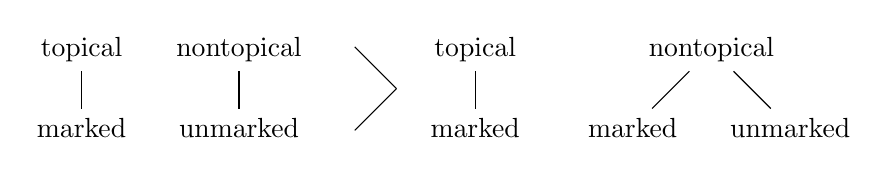
\begin{tikzpicture}
	\node (1) at (0,0) {topical};
	\node (12) at (0,-1) {marked};
	 \draw (1) -- (12);

\node (2) at (2,0) {nontopical};
	\node (22) at (2,-1) {unmarked};
	 \draw (2) -- (22);

 % \node (3) at (3.75,-0.5) {>};
\draw (4,-0.5) -- ++(135:.75cm);
\draw (4,-0.5) -- ++(225:.75cm);

\node (4) at (5,0) {topical};
	\node (41) at (5,-1) {marked};
	 \draw (4) -- (41);

\node (5) at (8,0) {nontopical};
\node (511) at (7,-1) {marked};
\node (512) at (9,-1) {unmarked};
	 \draw (5) -- (511);
\draw (5) -- (512);
\end{tikzpicture}
\end{exe}

\citet[215]{Dalrympleetal2011Objects} suggest that spreading accounts
for \citegen{Bresnanetal1987Topic} distinction between anaphoric and
agreement function of object markers in \ili{Bantu} languages: spreading
leads to the development of agreement-like properties. However, their
approach improves on both \citet{Bresnanetal1987Topic} and on
\citet{Creissels2006Typology} by making explicit the role of the
hierarchies in~\REF{02-do-ex:8} in motivating the marking of
only certain nontopicalized objects, leading to a DOM system. The
other scenario, schematized in~\REF{02-do-ex:33}, is for object marking to narrow. 
In this scenario, only a subset of topical objects
(those with features high on the \isi{topicality} hierarchies
in~\REF{02-do-ex:8} come to be marked, while other objects –
whether topical or nontopical – are unmarked:

\begin{exe}
\ex
\label{02-do-ex:33}%Chichewa
Narrowing of DOM \citet[218]{Dalrympleetal2011Objects}\\


\begin{tikzpicture}
	\node (1) at (0,0) {topical};
	\node (12) at (0,-1) {marked};
	 \draw (1) -- (12);

\node (2) at (2,0) {nontopical};
	\node (22) at (2,-1) {unmarked};
	 \draw (2) -- (22);

 % \node (3) at (3.75,-0.5) {>};
\draw (4,-0.5) -- ++(135:.75cm);
\draw (4,-0.5) -- ++(225:.75cm);

\node (5) at (6,0) {topical};
\node (511) at (5,-1) {marked};
\node (512) at (7,-1) {unmarked};
	 \draw (5) -- (511);
\draw (5) -- (512);

\node (4) at (9,0) {nontopical};
	\node (41) at (9,-1) {unmarked};
	 \draw (4) -- (41);
\end{tikzpicture}
\end{exe}

\ili{Chichewa} does not straightforwardly fit either of these scenarios, as
object marking both spreads and narrows in \ili{Chichewa}. Object marking
spreads to nontopical objects, if they are human and therefore high on
the \isi{topicality} hierarchies in~\REF{02-do-ex:8}. Object marking
also retracts from less topic-worthy objects, even if they are topical
(i.e., in a position outside of the clause). A more general problem
is that the second path – simple narrowing – is not consistent with
the proposal that object marking in \ili{Bantu} languages arises in stages
along an anaphor-agreement continuum \citep{Bresnanetal1987Topic,
 Creissels2006Typology, Givon1976Topic}.
\citegen{Creissels2006Typology} Stages~II and III preclude the
possibility of narrowing the object marking of anaphoric nominals
without also spreading object marking to indicate grammatical
agreement. And, indeed, I have not found any examples of simple
narrowing in the literature on \ili{Bantu} object marking. The assumption is
that object marking by default tracks topicalized (dislocated)
objects, while agreement-like marking is the more restricted
innovation. (See \eg \citealt{Riedel2009Syntax,Baxetal2012Information,
 Martenetal2012Object}.) However, narrowing of
object marking subsequent to spread can be seen as a logical
progression in the development of a grammatical agreement system from
an anaphoric one. What is missing from
\citegen{Dalrympleetal2011Objects} approach, then, is a way of placing
their \isi{grammaticalization} paths on an anaphor-agreement continuum.

\subsection{An alternative}
\label{Downing-Alternative}
In this section, I propose an alternative account of the
\isi{grammaticalization} of object marking in \ili{Chichewa} which combines
aspects of both \citegen{Creissels2006Typology} and
\citegen{Dalrympleetal2011Objects} approaches. Following
\citet{Iemmolo2013Symmetric,Iemmolo2014Differential}, 
I propose that in \ili{Chichewa} (and other \ili{Bantu} languages where object
marking is conditioned by the \isi{topicality} hierarchies) the object
marker is reinterpreted as marking topic-worthiness rather than
topic-hood. (Topic-worthy objects are ones with semantic features that
are high in the \isi{topicality} hierarchies.) Topic-worthy objects come to
be marked, whether they are topical or nontopical in information
structure or syntactic terms. Less topic-worthy objects are not
obligatorily marked, even if they are topical. That is,
topic-worthiness trumps both \isi{information structure} and syntax in
triggering the development of \ili{Bantu} agreement-like object marking
systems from purely anaphoric agreement systems.\footnote{As work
 since \citet{Comrie1981Language,Comrie1989Language} proposes, marking highly
 topic-worthy objects plausibly has a disambiguating function, since
 nominals high in the \isi{topicality} hierarchy are canonically subjects,
 rather than objects. See \citetv{Witzlacketal2017Differential} for further
 discussion.}

I formalize these observations in terms of the syntactic and semantic
constraints in~\REF{02-do-ex:34}. The syntactic ones are
adapted from observations in work like \citet{Bresnanetal1987Topic},
\citet{Morimoto2002Prominence}, \citet{Creissels2006Typology}
concerning the distribution of object markers. The semantic ones are
inspired by work like \citet{Aissen2003Differential},
\citet{Dalrympleetal2011Objects}, \citet{Iemmolo2013Symmetric,Iemmolo2014Differential} 
and \citet{Morimoto2002Prominence} on the role of topic-worthiness in
defining DOM.\footnote{See \citet{Morimoto2002Prominence} and
\citet{vanderWal2015Bantu} for recent proposals formalizing the agreement-anaphor continuum for
 \ili{Bantu} object marking in theoretical syntax frameworks. It is beyond
 the scope of this paper to critique these formal alternatives.}

{
\begin{exe}
\ex
\label{02-do-ex:34}
Constraints defining the development of DOM from a topic-marking system\\
\textit{syntactic}\footnote{As a reviewer points out, the combined syntactic constraints in~\REF{02-do-ex:34a}, \REF{02-do-ex:34b} bear a resemblance to the Theta Criterion in generative grammar \citet{Chomsky1981Lectures}: “Each argument bears one and only one theta-role, and each theta-role is assigned to one and only one argument.”} 
\begin{xlist}
\ex
\label{02-do-ex:34a}
*[Index\textsubscript{i}, NP\textsubscript{i}]\textsubscript{vP}:\\
Grammatical agreement with an overt in situ object nominal violates this constraint, as object marking with an overt in situ object (if identical in form to anaphoric use of \isi{object marker}) violates the condition that there should be only one expression of the object in the VP.
\ex
\label{02-do-ex:34b}
\textsc{Max argument/VP}:\\
Argument roles in the input VP must be realized overtly in the output VP \citep{Morimoto2002Prominence}. This constraint is violated if a topicalized object is not resumed with an \isi{object marker}.
\end{xlist}
\textit{semantic}
\begin{xlist}
\exi{c.}
\label{02-do-ex:34c}
*øIndex[+TW]:\\
Topic-worthy [+TW] objects should be indexed by object marking. \citet{Aissen2003Differential}\\
(Topic-worthiness is defined by the \isi{topicality} hierarchies in~\REF{02-do-ex:8}.)

\exi{d.}
\label{02-do-ex:34d}
*Index[-TW]:\\
Non-topic worthy [–TW] objects should not be indexed by object marking.
\end{xlist}
\end{exe}
}

Ranking the constraints in Optimality Theoretic style tableaux allows
one to use a factorial typology to formalize the steps in the
development of \ili{Bantu} DOM systems and to formalize the relative
importance of each constraint in defining stages along a
\isi{grammaticalization path}.

\subsubsection{Stage~I: purely anaphoric use of OM}
At \citegen{Creissels2006Typology} and \citegen{Dalrympleetal2011Objects} initial stage, object markers have a purely anaphoric function: object markers resume co-referential clause-external objects. This is optimal if the syntactic constraints in~\REF{02-do-ex:34} conditioning the distribution of object marking outrank the semantic constraints, as shown in Tableau~\REF{02-do-ex:35b}, using schematized syntactic structures.

\ea \label{02-do-ex:35} 
\begin{xlist}
\ex \label{02-do-ex:35a}
*[Index\textsubscript{i}, NP\textsubscript{i}]\textsubscript{vP} >> \textsc{Max arg(ument)/VP} >> *øIndex[+TW] >> \mbox{*Index[-TW]}

\exbox{ \label{02-do-ex:35b}
\resizebox{1.1\linewidth}{!}{
\begin{tabular}[t]{r|l|c|c|c|c|}
\cline{2-6}
     &   & *[Index$_i$, NP$_i$]\textsubscript{vP} & \textsc{Max arg/VP} & *øIndex[+TW]   & *Index[-TW]   \\
\LCC 
      &       &       & \white & &  \\
\cline{2-6}
\hand & 1. NP$_i$ [S [V- OM$_i$] &       &    & &   *     \\ 
\cline{2-6}
      & 2. NP$_i$ [S [V- øi] &     &  *!   & * &        \\
\cline{2-6}
 \addlinespace[.04em]
\cline{2-6} 
 \addlinespace[-.04em]
%         \specialrule{2.5pt}{1pt}{1pt}
\hand & 3. [S [V- OM$_i$ NP$_i$]   &  *!     &    & &    *    \\ 
\cline{2-6}
      & 4. [S [V NP$_i$]  &     &     &* &        \\
\cline{2-6}
\ECC
\end{tabular}
}
}
\end{xlist}
\z

Object marking is optimal when an object NP is dislocated: this is shown by candidate~\REF{02-do-ex:35b}-1. Omitting object marking to resume the dislocated object, as in candidate~\REF{02-do-ex:35b}-2, violates \textsc{Max arg(ument)/VP}, the constraint requiring an overt realization of the object within the VP. This ranking of the constraints defines agreement as non-optimal, however. As we can see, candidate~\REF{02-do-ex:35b}-3, with a coreferential \isi{object marker} resuming an object within the VP, violates *[Index\textsubscript{i}, NP\textsubscript{i} ]\textsubscript{vP}.

\subsubsection{Step 1 in the development of DOM} 
The first step in the development of a DOM system involves
\textit{spreading} of object marking to non-topicalized objects which
are semantically topic-worthy [+TW]. This becomes optimal when the
semantic constraint requiring marking of [+TW] objects~\REF{02-do-ex:34c}
comes to outrank the two syntactic constraints~\REF{02-do-ex:34a}–\REF{02-do-ex:34b};
re-ranked constraints are bolded:

\ea
\label{02-do-ex:36}
DOM of in situ objects is optimal with ranking,\\
*øIndex[+TW] >> *[Index\textsubscript{i}, NP\textsubscript{i}]\textsubscript{vP} >> \textsc{Max arg(ument)/VP} >> *Index[-TW] 
\z

\ili{Swahili} exemplifies this kind of \ili{Bantu} object marking system. Recall
from \sectref{02-do-sec:2-2} that in
\ili{Swahili}, we find object marking with all topicalized objects and
grammatical agreement only with [+TW] objects. 
Tableaux~\REF{02-do-ex:37} exemplify this next step in the DOM \isi{grammaticalization path}.

\ea \label{02-do-ex:37}
\ea \label{02-do-ex:37a}
Object NP is [+TW]

\resizebox{\linewidth}{!}{
\begin{tabular}[t]{r|l|c|c|c|c|}
\cline{2-6}
& & *øIndex[+TW]	& *[Index\textsubscript{i}, NP\textsubscript{i}]\textsubscript{vP} & \textsc{Max arg/VP} & *Index[-TW]\\\cline{2-6}
\hand & 1. NP\textsubscript{i} [S [V-OM\textsubscript{i}] & & & &\\\cline{2-6}
& 2. NP\textsubscript{i} [S [V- øi] & & *! & * &\\

\cline{2-6}
 \addlinespace[.04em]
\cline{2-6} 
 \addlinespace[-.04em]

\hand & 3. [S [V- OM\textsubscript{i} NP\textsubscript{i}] & & * & &\\\cline{2-6}
& 4. [S [V NP\textsubscript{i}] & *! & & &\\\cline{2-6}
\end{tabular}
}

\newpage   
\ex \label{02-do-ex:37b}
Object NP is [-TW]\\ 
\resizebox{\linewidth}{!}{
\begin{tabular}[t]{r|l|c|c|c|c|}
\cline{2-6}
& & *øIndex[+TW]	& *[Index\textsubscript{i}, NP\textsubscript{i}]\textsubscript{vP} & \textsc{Max arg/VP} & *Index[-TW]\\\cline{2-6}
\hand & 1. NP\textsubscript{i} [S [V-OM\textsubscript{i}] & & & & *\\\cline{2-6}
& 2. NP\textsubscript{i} [S [V- øi] & & & *! &\\
\cline{2-6} \addlinespace[.04em]\cline{2-6}  \addlinespace[-.04em]
& 3. [S [V- OM\textsubscript{i} NP\textsubscript{i}] & & *! & & *\\\cline{2-6}
\hand & 4. [S [V NP\textsubscript{i}] & & & &\\\cline{2-6}
\end{tabular}
}
\z
\z

Tableaux~\REF{02-do-ex:37a} and \REF{02-do-ex:37b} demonstrate that the anaphoric use
of object marking remains optimal both when a [+TW] object is
topicalized and when a [–TW] object is topicalized. This context is
illustrated by candidates \REF{02-do-ex:37a}-1 and
\REF{02-do-ex:37b}-1. Candidate \REF{02-do-ex:37a}-3 shows that when the
semantic constraint \textbf{*øIndex[+TW]} is high ranked, object
marking in the agreement context is optimal for a [+TW]
object. However, object marking remains non-optimal in the agreement
context for a [–TW] object, as shown by candidate \REF{02-do-ex:37b}-3.\\

\subsubsection{Step 2: modern colloquial Chichewa}
As noted above, it is problematic to account for DOM in modern
colloquial \ili{Chichewa} using
\citeauthor{Dalrympleetal2011Objects}’s (\citeyear{Dalrympleetal2011Objects}) 
\isi{grammaticalization} paths, as we find both \textit{spreading} of
marking (to non-topical topic-worthy objects) and \textit{narrowing}
of marking from non-topic worthy topicalized objects. The
constraint-based approach developed here can straightforwardly
formalize this second step by ranking the second semantic
constraint~\REF{02-do-ex:34d} higher than the second syntactic
constraint~\REF{02-do-ex:34b}:

\ea \label{02-do-ex:38}
*øIndex[+TW] >> *[Index\textsubscript{i}, NP\textsubscript{i}]\textsubscript{vP} >> *Index[-TW] >> \textsc{Max arg(ument)/VP}
\end{exe}
This is exemplified in Tableaux~\REF{02-do-ex:39}:
 
\begin{exe}
\ex
\label{02-do-ex:39}
\begin{xlist}
\ex
\label{02-do-ex:39a}

Object NP is [+ TW]\\
\resizebox{\linewidth}{!}{
\begin{tabular}[t]{r|l|c|c|c|c|}
\cline{2-6}
& & *øIndex[+TW]	& *[Index\textsubscript{i}, NP\textsubscript{i}]\textsubscript{vP} & *Index[-TW] & \textsc{Max arg/VP}\\\cline{2-6}
\hand & 1. NP\textsubscript{i} [S [V-OM\textsubscript{i}] & & & &\\\cline{2-6}
& 2. NP\textsubscript{i} [S [V- øi] & *! & & & *\\
\cline{2-6} \addlinespace[.04em]\cline{2-6}  \addlinespace[-.04em]
\hand & 3. [S [V- OM\textsubscript{i} NP\textsubscript{i}] & & * & &\\\cline{2-6}
& 4. [S [V NP\textsubscript{i}] & *! & & &\\\cline{2-6}
\end{tabular}}  
\medskip
\ex
\label{02-do-ex:39b} 
Object NP is [-TW]\\
\resizebox{\linewidth}{!}{
\begin{tabular}[t]{r|l|c|c|c|c|}
\cline{2-6}
& & *øIndex[+TW]	& *[Index\textsubscript{i}, NP\textsubscript{i}]\textsubscript{vP} & *Index[-TW] & \textsc{Max arg/VP}\\\cline{2-6}
\hand & 1. NP\textsubscript{i} [S [V-OM\textsubscript{i}] & & & *! &\\\cline{2-6}
& 2. NP\textsubscript{i} [S [V- øi] & & & & *\\
\cline{2-6} \addlinespace[.04em]\cline{2-6}  \addlinespace[-.04em]
\hand & 3. [S [V- OM\textsubscript{i} NP\textsubscript{i}] & & *! & * &\\\cline{2-6}
& 4. [S [V NP\textsubscript{i}] & & & &\\\cline{2-6}
\end{tabular}}
\end{xlist}
\end{exe} 
Tableaux in~\REF{02-do-ex:39a} and \REF{02-do-ex:39b} show that with this
constraint ranking, anaphoric use of object marking is only optimal
when a [+TW] object NP is dislocated: candidate
\REF{02-do-ex:39a}-1. Candidate \REF{02-do-ex:39b}-1, with object marking on a
dislocated [-TW] object violates the semantic constraint,
*Index[-TW]. Similarly, object marking is also optimal in the
agreement context only with a [+TW] object: candidate
\REF{02-do-ex:39a}-3. Object marking on a [-TW] object in the agreement
context, candidate \REF{02-do-ex:39b}-3, violates the syntactic constraint, *[Index\textsubscript{i}, NP\textsubscript{i}
 ]\textsubscript{vP}.\footnote{As a reviewer points out, the
 analysis developed here does not account for the variation we find
 in \ili{Chichewa}. 
 Object marking is possible with all dislocated objects,
 even non-topic-worthy ones. 
 The DOM restriction is therefore a
 tendency, not an absolute. How best to formalize this variation is a
 topic for future research.}

\subsubsection{Accounting for gaps}
A further advantage of this constraints-based approach is that it can
account for gaps in the cross-\ili{Bantu} object marking data. 
As noted
above, we do not find the simple narrowing of marking of topicalized
object which \citet{Dalrympleetal2011Objects} propose as an alternative
\isi{grammaticalization path}, as schematized in~\REF{02-do-ex:33}. 
Indeed,
we noted that if DOM in \ili{Bantu} languages results from change along an
anaphor-agreement continuum, we do not expect simple narrowing, and we would want to account for this. 
What I propose is that this direction
of change falls out if the two syntactic constraints \REF{02-do-ex:40a} and the two topicality-sensitive constraints \REF{02-do-ex:40b} have the harmonic alignment rankings shown in~\REF{02-do-ex:40}:

\begin{exe}
\ex
\label{02-do-ex:40}%Chichewa
Harmonic alignment
\begin{xlist}
\ex
\label{02-do-ex:40a}%Chichewa
*[Index\textsubscript{i}, NP\textsubscript{i}]\textsubscript{vP} >> \textsc{Max arg(ument)/VP}
\ex
\label{02-do-ex:40b}%Chichewa
*øIndex[+TW] >> *Index[-TW]
\end{xlist}
\end{exe}

A harmonic alignment ranking cannot be reordered to define a typology \citep{Aissen2003Differential,Morimoto2002Prominence}. As we can see in Tableaux in~\REF{02-do-ex:42}, narrowing without spreading (\cf \REF{02-do-ex:32} and \REF{02-do-ex:33}, above) is only optimal given the ranking in~\REF{02-do-ex:41}, which violates the harmonic ranking of the semantic constraints defined in~\REF{02-do-ex:40b}.

\ea \label{02-do-ex:41}%Chichewa
*[Index\textsubscript{i}, NP\textsubscript{i}]\textsubscript{vP} , *Index[-TW] >> \textsc{Max arg(ument)/VP} >> *øIndex[+TW]
\z
 
\ea \label{02-do-ex:42}
\ea \label{02-do-ex:42a}
Object NP is [+TW]\\
\resizebox{\linewidth}{!}{
\begin{tabular}[t]{r|l|c:c|c|c|}
\cline{2-6}
& & *[Index\textsubscript{i}, NP\textsubscript{i}]\textsubscript{vP} & *Index[-TW] & \textsc{Max arg/VP} & *øIndex[+TW]\\\cline{2-6}
\hand & 1. NP\textsubscript{i} [S [V-OM\textsubscript{i}] & & & &\\\cline{2-6}
& 2. NP\textsubscript{i} [S [V- øi] & & & *! & *\\\cline{2-6}
\cline{2-6} \addlinespace[.04em]\cline{2-6}  \addlinespace[-.04em]
& 3. [S [V- OM\textsubscript{i} NP\textsubscript{i}] & *! & & &\\\cline{2-6}
\hand & 4. [S [V NP\textsubscript{i}] & & & & *\\\cline{2-6}
\end{tabular}}
 
\ex \label{02-do-ex:42b}
Object NP is [-TW]

\resizebox{\linewidth}{!}{
\begin{tabular}[t]{r|l|c:c|c|c|}
\cline{2-6}
& & *[Index\textsubscript{i}, NP\textsubscript{i}]\textsubscript{vP} & *Index[-TW] & \textsc{Max arg/VP} & *øIndex[+TW]\\\cline{2-6}
& 1. NP\textsubscript{i} [S [V-OM\textsubscript{i}] & & *! & &\\\cline{2-6}
\hand & 2. NP\textsubscript{i} [S [V- øi] & & & * &\\\cline{2-6}
\cline{2-6} \addlinespace[.04em]\cline{2-6}  \addlinespace[-.04em]
& 3. [S [V- OM\textsubscript{i} NP\textsubscript{i}] & *! & * & &\\\cline{2-6}
\hand & 4. [S [V NP\textsubscript{i}] & & & &\\\cline{2-6}
\end{tabular}}
\z
\z

Comparing the first candidates in Tableaux~\REF{02-do-ex:42a} and
\REF{02-do-ex:42b} allows one to see that this constraint ranking optimizes narrowing. 
Anaphoric use of object marking is optimal only when a [+TW] object is dislocated, as in candidate \REF{02-do-ex:42a}-1, %TODO [cmld] Angabe der Kandidaten so ok? Ich wollte zeigen, dass, wie gewöhnlich, das in Klammern die Beispielnummer ist und die Kandidatennummer kommt dann danach.
 but not when a [–TW] object is dislocated, as in candidate \REF{02-do-ex:42b}-1. Note that candidate \REF{02-do-ex:42b}-1 violates the semantic constraint, *Index[-TW]. 
Object marking in the agreement context is not optimal,
whether the object is topic-worthy or not, as this violates the
syntactic constraint, *[Index\textsubscript{i}, NP\textsubscript{i}
]\textsubscript{vP}. Candidates \REF{02-do-ex:42a}-3 and \REF{02-do-ex:42b}-3
illustrate this. While this ranking clearly can define narrowing, it
violates the harmonic ranking of the semantic constraints. Finally,
the constraints-based approach can explain why
\citet{Creissels2006Typology} says he finds no examples of his
Stage~III: a purely grammatical agreement system for object marking
which ignores the topicworthiness of the object. To make this kind of
agreement system optimal, we must introduce a new semantic constraint, *øIndex[ TW], which clearly contradicts the better motivated
constraint: *Index[–TW]. This new constraint, highly ranked, optimizes
object marking on both topicworthy and non-topicworthy objects in the
agreement context:

\begin{exe}
\ex
\label{02-do-ex:43}
*øIndex[+TW] >> *øIndex[-TW] >> *[Index\textsubscript{i}, NP\textsubscript{i}]\textsubscript{vP} >> \textsc{Max arg(ument)/VP} \\
>> *Index[-TW]
\end{exe}

However, as Tableau~\REF{02-do-ex:44} exemplifies, this same ranking cannot define \citegen{Creissels2006Typology} Stage~III, because it incorrectly optimizes object marking to resume topicalized objects:

  
\begin{exe}
\ex
\label{02-do-ex:44}
Object NP is either [+TW] or [-TW]
 
\resizebox{\linewidth}{!}{
\begin{tabular}[t]{r|l|c|c|c|c|c|}
\cline{2-7}
& & *øIndex[+TW] & *øIndex[-TW] & *[Index\textsubscript{i}, NP\textsubscript{i}]\textsubscript{vP} & \textsc{Max arg/VP} & *Index[-TW]\\\cline{2-7}
\hand & a. NP\textsubscript{i} [S [V-OM\textsubscript{i}] & & & & * &\\\cline{2-7}
& b. NP\textsubscript{i} [S [V- øi] & *! & * & & * & *\\\cline{2-7}
\hand & c. [S [V- OM\textsubscript{i} NP\textsubscript{i}] & & & & & *\\\cline{2-7}
& d. [S [V NP\textsubscript{i}] & *! & * & & &\\\cline{2-7}
\end{tabular}}
\end{exe} 
Tableau \REF{02-do-ex:44} shows that these constraints and this ranking optimize agreement with any co-referential object, whether topicalized (candidates \REF{02-do-ex:44}-a and \REF{02-do-ex:44}-b) or in a grammatical agreement context (candidates \REF{02-do-ex:44}-c and \REF{02-do-ex:44})-d. 
Stage~III, therefore, is not found because it is not optimal under any ranking of the proposed constraints that define a \isi{grammaticalization path} leading to a DOM system.

\section{Conclusion}
\label{Downing-Conclusion}
As we have seen, object markers are not
“purely anaphoric” in modern colloquial \ili{Chichewa}. They are also not pure agreement markers, as they
occur only variably (not obligatorily), and they only co-occur with
clause-internal human objects. Rather, their distribution conforms to
\citegen{Bentley1994Syntactic}, \citegen{Morimoto2002Prominence},
\citegen{Riedel2009Syntax}, \citegen{Martenetal2012Object}’s and
\citegen{vanderWal2015Bantu} observation that the occurrence of grammatical agreement-like object markers in \ili{Bantu} languages is conditioned by the hierarchies in~\REF{02-do-ex:8}. 
As a result, in \ili{Chichewa}, as in many \ili{Bantu} languages, we find a DOM system. 
Following \citet{Iemmolo2013Symmetric,Iemmolo2014Differential} I have proposed that the \isi{grammaticalization path} towards DOM is for object markers to come to index not just topic-hood (an information
structural and/or syntactic property) but also topic-worthiness (a
semantic property). In \ili{Chichewa}, as I have shown, topic-worthiness is
quite systematically indexed. This observation forms the basis for a
constraints-based account of the development of DOM in \ili{Bantu}
languages, which improves on \citet{Creissels2006Typology} by
incorporating the notion of topic-worthiness as a trigger for the
movement from anaphoric agreement to grammatical agreement. 
It improves on \citet{Dalrympleetal2011Objects} by providing a way of
formalizing the anaphor-agreement continuum that is central to the
discussion of the development of DOM in \ili{Bantu} languages. 
It is hoped this proposal provides a useful basis for a more comprehensive study of the DOM properties of object marking in \ili{Bantu} languages.


\section*{Acknowledgements}
I would first like to thank my \ili{Chichewa} language consultants for their
patience in helping me learn about their language, and in addition, Al
Mtenje and Pascal Kishindo for helpful discussion. I am grateful to
the Centre for Language Studies, University of Malawi, for their
hospitality during my 2011, 2013 and 2015 visits to Malawi. Earlier
versions of this talk were presented at the Paris BANTUPSYN workshop
in June 2012, a GU GRAM:SEM colloquium in 2013, CALL 2013, the DAM
Workshop, and ACAL45. I thank those audiences for useful feedback, in
particular Lisa Cheng, Elisabet Engdahl, Giorgio Iemmolo, Liz Coppock,
Klaus van Heusinger, Kristina Riedel and Thilo Schadeberg. Responding
to thoughtful comments by the editors of the volume and an anonymous
reviewer has improved both the content and presentation of the
analysis. This research has been supported by the ANR-DFG
French-German cooperative grant BANTUPSYN and by Göteborgs universitet travel grants.

\section*{Abbreviations}

\begin{tabularx}{.45\textwidth}{lQ}
1 & first person\\
2 & second person\\
3 & third person\\
\textsc{cl} & noun class concord affixes (\eg cl1, cl2, etc.)\\
\textsc{cop} & copula\\
\textsc{dem} & demonstrative\\
\textsc{emph} & emphasis\\
\textsc{fut} & future\\
\textsc{fv} & final vowel\\
\textsc{hab} & habitual\\
\textsc{inf} & infinitive\\
\end{tabularx}
\begin{tabularx}{.45\textwidth}{lQ}
\textsc{loc} & locative\\
\textsc{obj} & object\\
\textsc{pl} & plural\\
\textsc{poss} & possessive\\
\textsc{prf} & perfect\\
\textsc{prog} & progressive\\
\textsc{pst} & past\\
\textsc{q} & question marker\\
\textsc{rel} & relative\\
\textsc{sbj} & subject\\
\textsc{sg} & singular\\
\\
\end{tabularx}

{\sloppy
\printbibliography[heading=subbibliography,notkeyword=this] }
\end{document}

